%PERCENTS AS RATES PER 100 - WORKSHEET 0 (IN-CLASS INSTRUCTION)
\documentclass[12pt, letterpaper, fleqn]{article}

% ----------------------------------------------------------
% PACKAGES
% ----------------------------------------------------------
\usepackage{graphicx}
\usepackage{xcolor}
\usepackage[most]{tcolorbox}
\usepackage{amsmath, amssymb}
\usepackage{fancyhdr}
\usepackage[utf8]{inputenc}
\usepackage[T1]{fontenc}
\usepackage{enumitem}
\usepackage{geometry}
\usepackage{tikz}
\usepackage{needspace}
\usepackage{multicol}

\usetikzlibrary{arrows.meta, calc}

% ----------------------------------------------------------
% PAGE SETUP
% ----------------------------------------------------------
\usepackage{times}
\geometry{letterpaper, top=1.25in, bottom=1.25in, marginpar=0.5in}

% ----------------------------------------------------------
% HEADER / FOOTER
% ----------------------------------------------------------
\newcommand{\logowidth}{3cm}
\setlength{\headheight}{20pt}
\setlength{\footskip}{40pt}

\pagestyle{fancy}
\fancyhf{}
\fancyhead[C]{\small\bfseries Percents as Rates per 100}
\fancyfoot[L]{\raisebox{2pt}{
\includegraphics[width=\logowidth]{kss.png}}}
\fancyfoot[C]{\thepage}
\fancyfoot[R]{6.4.0}

\renewcommand{\footrulewidth}{0.2pt}

% ----------------------------------------------------------
% THEME COLOR
% ----------------------------------------------------------
\definecolor{customteal}{HTML}{2fbdb9}

% ----------------------------------------------------------
% HELPER MACROS
% ----------------------------------------------------------
\newcommand{\blank}{\underline{\hspace{2.2cm}}}
\newcommand{\blanklong}{\underline{\hspace{6.5cm}}}
\newcommand{\blankshorter}{\underline{\hspace{1.5cm}}}

% ----------------------------------------------------------
% DOCUMENT
% ----------------------------------------------------------
\begin{document}


\textbf{Name:} \underline{\hspace{5cm}}
\hfill
\textbf{Date:} \underline{\hspace{3cm}}\\

% ==========================================================
% SECTION 1: WHAT IS A PERCENT?
% ==========================================================
\begin{tcolorbox}[colback=customteal!20]
    \large\textcolor{black}{\textbf{What is a Percent? (Foundation)}}
\end{tcolorbox}

\vspace{3mm}

\noindent
The word ``percent'' means ``per hundred.'' A \textbf{percent} is a ratio that compares a number to 100.

\vspace{0.5cm}

\begin{itemize}
    \item 25\% means $\dfrac{25}{100}$ or ``25 out of every 100''
    \item 50\% means $\dfrac{50}{100}$ or ``50 out of every 100''
    \item 100\% means $\dfrac{100}{100}$ or ``all of it''
    \item 0\% means $\dfrac{0}{100}$ or ``none of it''
\end{itemize}


\vspace{1.5cm}

\noindent
\textbf{Key Insight:} A percent is just a rate with denominator 100!

\vspace{1.5cm}
% ==========================================================
% VISUAL REPRESENTATION
% ==========================================================
\begin{tcolorbox}[colback=white, colframe=black!25, boxrule=0.6pt, arc=4mm, left=6mm, right=6mm, top=5mm, bottom=5mm]


\textbf{Example: 40\% Shaded}
\vspace{1cm}
\begin{center}
\begin{tikzpicture}[scale=0.8]
% Shade only first 4 cells
\foreach \x in {0,1,2,3} {
    \draw[fill=black!50] (\x,0) rectangle (\x+1,1);
}
% Draw grid on top so borders show over fill
\draw[thick, step=1] (0,0) grid (10,1);
\medskip

\node at (5, -0.5) {4 out of 10 squares are shaded}; 
\vspace{1cm}

\node at (5, -1.0) {This is 40\%};
\end{tikzpicture}
\end{center}
\vspace{1cm}
\end{tcolorbox}

\vspace{4mm}

\newpage

% ==========================================================
% ADDITION 1: INSERT IN SECTION 1 (WHAT IS A PERCENT?)
% RIGHT AFTER THE "KEY INSIGHT" BOX TO TEACH SCALING
% ==========================================================

\begin{tcolorbox}[colback=white, colframe=black!25, boxrule=0.6pt, arc=4mm, left=6mm, right=6mm, top=5mm, bottom=5mm]

\textbf{How to Convert Fractions with Bases other than 100:}

\noindent
If a fraction does not have 100 as its denominator, find an equivalent fraction by multiplying or dividing to get a denominator of 100.

\vspace{0.3cm}

\begin{align*}
\text{\textbf{Scale Up:}} \quad \dfrac{4}{5} &= \dfrac{4 \times 20}{5 \times 20} = \dfrac{80}{100} = 80\% \\ \\
\text{\textbf{Scale Down:}} \quad \dfrac{42}{300} &= \dfrac{42 \div 3}{300 \div 3} = \dfrac{14}{100} = 14\%
\end{align*}

\end{tcolorbox}

\vspace{4mm}


% ==========================================================
% PRACTICE 1: RECOGNIZING PERCENTS
% ==========================================================
\begin{tcolorbox}[colback=customteal!20]
\large\textcolor{black}{\textbf{Practice: Write Fractions as Percents}}
\end{tcolorbox}

\noindent
Convert each fraction to a percent.

\vspace{1.5cm}

\begin{multicols}{2}
\begin{enumerate}[itemsep=1.2cm, leftmargin=0.6cm]
\item $\dfrac{50}{100} = $ \blankshorter \; \%
\vspace{1.5cm}
\item $\dfrac{75}{100} = $ \blankshorter \; \%
\vspace{1.5cm}
\item $\dfrac{5}{100} = $ \blankshorter \; \%
\vspace{1.5cm}
\item $\dfrac{4}{5} = $ \blankshorter \; \%
\vspace{1.5cm}
\item $\dfrac{18}{20} = $ \blankshorter \; \%
\vspace{1.5cm}
\item $\dfrac{150}{300} = $ \blankshorter \; \%
\vspace{1.5cm}

\end{enumerate}
\end{multicols}

\newpage



% ==========================================================
% SECTION 2: FINDING A PERCENT OF A QUANTITY
% ==========================================================
\begin{tcolorbox}[colback=customteal!20]
\large\textcolor{black}{\textbf{Finding a Percent of a Quantity}}
\end{tcolorbox}

\noindent
To find \textbf{a percent of a quantity}, multiply the percent (as a decimal) by the quantity.

\vspace{3mm}

\begin{tcolorbox}[colback=white, colframe=black!25, boxrule=0.6pt, arc=4mm, left=6mm, right=6mm, top=5mm, bottom=5mm]

\textbf{Worked Example 1: Finding a Percent of a Number}

\medskip

\textbf{Problem:} What is 25\% of 80?

\medskip

\noindent
\textbf{Solution:}

\begin{enumerate}
    \item Convert the percent to a decimal: $25\% = 0.25$
    
    \item Multiply by the quantity: $0.25 \times 80 = 20$
    
    \item Answer: 25\% of 80 is \textbf{20}
\end{enumerate}

\medskip

\noindent
\textbf{Check:} $\dfrac{20}{80} = \dfrac{1}{4} = \dfrac{25}{100} = 25\%$ 

\end{tcolorbox}

\vspace{4mm}

% ==========================================================
% PRACTICE 2: PERCENT OF A QUANTITY
% ==========================================================
\begin{tcolorbox}[colback=customteal!20]
\large\textcolor{black}{\textbf{Practice: Find the Percent}}
\end{tcolorbox}

\noindent
Find each percent. Show your work.

\vspace{3mm}

\begin{enumerate}[itemsep=1.5cm, leftmargin=0.6cm]

\item 10\% of 50 = \blank

\item 50\% of 200 = \blank

\item 20\% of 150 = \blank

\end{enumerate}

\newpage

% ==========================================================
% SECTION 3: FINDING THE WHOLE GIVEN PART AND PERCENT
% ==========================================================
\begin{tcolorbox}[colback=customteal!20]
\large\textcolor{black}{\textbf{Finding the Whole Given a Part and Percent}}
\end{tcolorbox}

\noindent
Sometimes you know the part and the percent, and need to find the whole. Use this formula:

$$\text{Part} = \text{Percent} \times \text{Whole}$$
\vspace{2mm}

\noindent
Rearranged: $\text{Whole} = \dfrac{\text{Part}}{\text{Percent}}$

\vspace{3mm}

\begin{tcolorbox}[colback=white, colframe=black!25, boxrule=0.6pt, arc=4mm, left=6mm, right=6mm, top=5mm, bottom=5mm]

\textbf{Worked Example 2: Finding the Whole}

\medskip

\textbf{Problem:} 20 is 50\% of what number?

\medskip

\noindent
\textbf{Solution:}

\medskip

\noindent
Whole $= \dfrac{\text{Part}}{\text{Percent}} = \dfrac{20}{0.50} = 40$

\medskip

\noindent
\textbf{Answer:} 20 is 50\% of \textbf{40}

\medskip

\noindent
\textbf{Check:} $0.50 \times 40 = 20$ 

\end{tcolorbox}

\vspace{4mm}

% ==========================================================
% THINKING PROBLEM 1
% ==========================================================
\begin{tcolorbox}[colback=white!15, colframe=black, boxrule=1.5pt, arc=4mm, left=6mm, right=6mm, top=5mm, bottom=5mm]

\textbf{Deeper Thinking Problem 1: Store Discount}

\medskip

\noindent
A store is having a 25\% off sale. An item originally costs \$80.

\noindent
\textbf{a)} How much money do you save?

\vspace{2.7cm}

\noindent
\textbf{b)} What is the sale price (the amount you pay)?

\vspace{2.7cm}

\end{tcolorbox}

\newpage

\begin{tcolorbox}[colback=customteal!20]
    \large\textcolor{black}{\textbf{Percent Increase, Decrease, and Tax}}
\end{tcolorbox}

\vspace{3mm}

\begin{itemize}
    \item \textbf{Percent Increase (or Tax / Markup):} Find the percentage amount and \textbf{add} it to the original value ($100\% + \text{Percent}$).
    \item \textbf{Percent Decrease (or Discount / Depreciation):} Find the percentage amount and \textbf{subtract} it from the original value ($100\% - \text{Percent}$).
\end{itemize}

\vspace{3mm}

\begin{tcolorbox}[colback=white, colframe=black!25, boxrule=0.6pt, arc=4mm, left=6mm, right=6mm, top=5mm, bottom=5mm]

\textbf{Worked Example: Total Bill with Tip}

\medskip
\textbf{Problem:} A meal costs \$50. You want to leave a 20\% tip. What is the total?
\medskip

\noindent
\textbf{Step 1:} Find the tip amount: $0.20 \times \$50 = \$10$ \\
\textbf{Step 2:} Add it to the original amount: $\$50 + \$10 = \$60$ \\
\textbf{Alternative Direct Method:} Total = $120\%$ of \$50 $\rightarrow 1.20 \times 50 = \$60$

\end{tcolorbox}

\vspace{4mm}

% ==========================================================
% SECTION 4: FINDING A PERCENT (PART ÷ WHOLE)
% ==========================================================
\begin{tcolorbox}[colback=customteal!20]
\large\textcolor{black}{\textbf{Finding What Percent One Number is of Another}}
\end{tcolorbox}

\noindent
To find \textbf{what percent} one number is of another, divide the part by the whole, then convert to a percent.

$$\text{Percent} = \dfrac{\text{Part}}{\text{Whole}} \times 100\%$$

\vspace{3mm}

\begin{tcolorbox}[colback=white, colframe=black!25, boxrule=0.6pt, arc=4mm, left=6mm, right=6mm, top=5mm, bottom=5mm]

\textbf{Worked Example 3: Finding the Percent}

\medskip

\textbf{Problem:} What percent of 50 is 15?

\medskip

\noindent
\textbf{Solution:}

\medskip

\noindent
Percent $= \dfrac{15}{50} \times 100\% = 0.30 \times 100\% = 30\%$

\medskip

\noindent
\textbf{Answer:} 15 is \textbf{30\%} of 50

\medskip

\noindent
\textbf{Check:} $0.30 \times 50 = 15$ $\checkmark$

\end{tcolorbox}

\vspace{4mm}

% ==========================================================
% THINKING PROBLEM 2
% ==========================================================
\begin{tcolorbox}[colback=white!15, colframe=black, boxrule=1.5pt, arc=4mm, left=6mm, right=6mm, top=5mm, bottom=5mm]

\textbf{Deeper Thinking Problem 2: Test Scores}

\medskip

\noindent
A student answers 18 questions correctly out of 20 on a test.

\noindent
\textbf{a)} What percent did the student get correct?

\vspace{3cm}

\noindent
\textbf{b)} What percent did the student get wrong?

\vspace{3cm}

\end{tcolorbox}

% ==========================================================
% THINKING PROBLEM 3
% ==========================================================
\begin{tcolorbox}[colback=white!15, colframe=black, boxrule=1.5pt, arc=4mm, left=6mm, right=6mm, top=5mm, bottom=5mm]

\textbf{Deeper Thinking Problem 3: Multi-Step Percent Problem}

\medskip

\noindent
A video game costs \$60. It goes on sale for 30\% off.

\vspace{1cm}

\noindent
\textbf{a)} How much is the discount (30\% of \$60)?

\vspace{2cm}

\noindent
\textbf{b)} What is the new price after the discount?

\vspace{2cm}

\noindent
\textbf{c)} If the store then adds a 10\% sales tax to the discounted price, what is the final amount you pay?

\vspace{2cm}

\end{tcolorbox}


\end{document}
\end{document}
